\section{Experiments}\label{experiments}

\subsection{Experimental Snapshot}\label{experimental-snapshot}

This section instantiates the generic benchmarking pipeline described in Section~\ref{method} under one fixed experimental configuration. All experiments reported in this paper were generated within a single internally consistent benchmark snapshot so that dataset preparation, model evaluation, and cross-dataset comparison remain directly comparable. The objective of this setup is to demonstrate the practical use of the proposed pipeline for local embedding-model selection rather than to claim universal superiority for any one model.

The experimental design follows a reusable decision-support pattern. A practitioner first defines one or more local document collections, applies the same preprocessing and benchmark-construction procedure to each collection, and evaluates the same candidate model roster under one shared setup. As shown in Figure~\ref{fig:experiment_snapshot_design}, this process yields repeated dataset-level benchmark outputs for each corpus before any higher-level comparison is attempted. The aggregate comparison stage is then constructed from these completed per-dataset outputs rather than from an alternative evaluation branch. In this paper, the design is instantiated with three corpora and five embedding models.

\begin{figure}
\centering
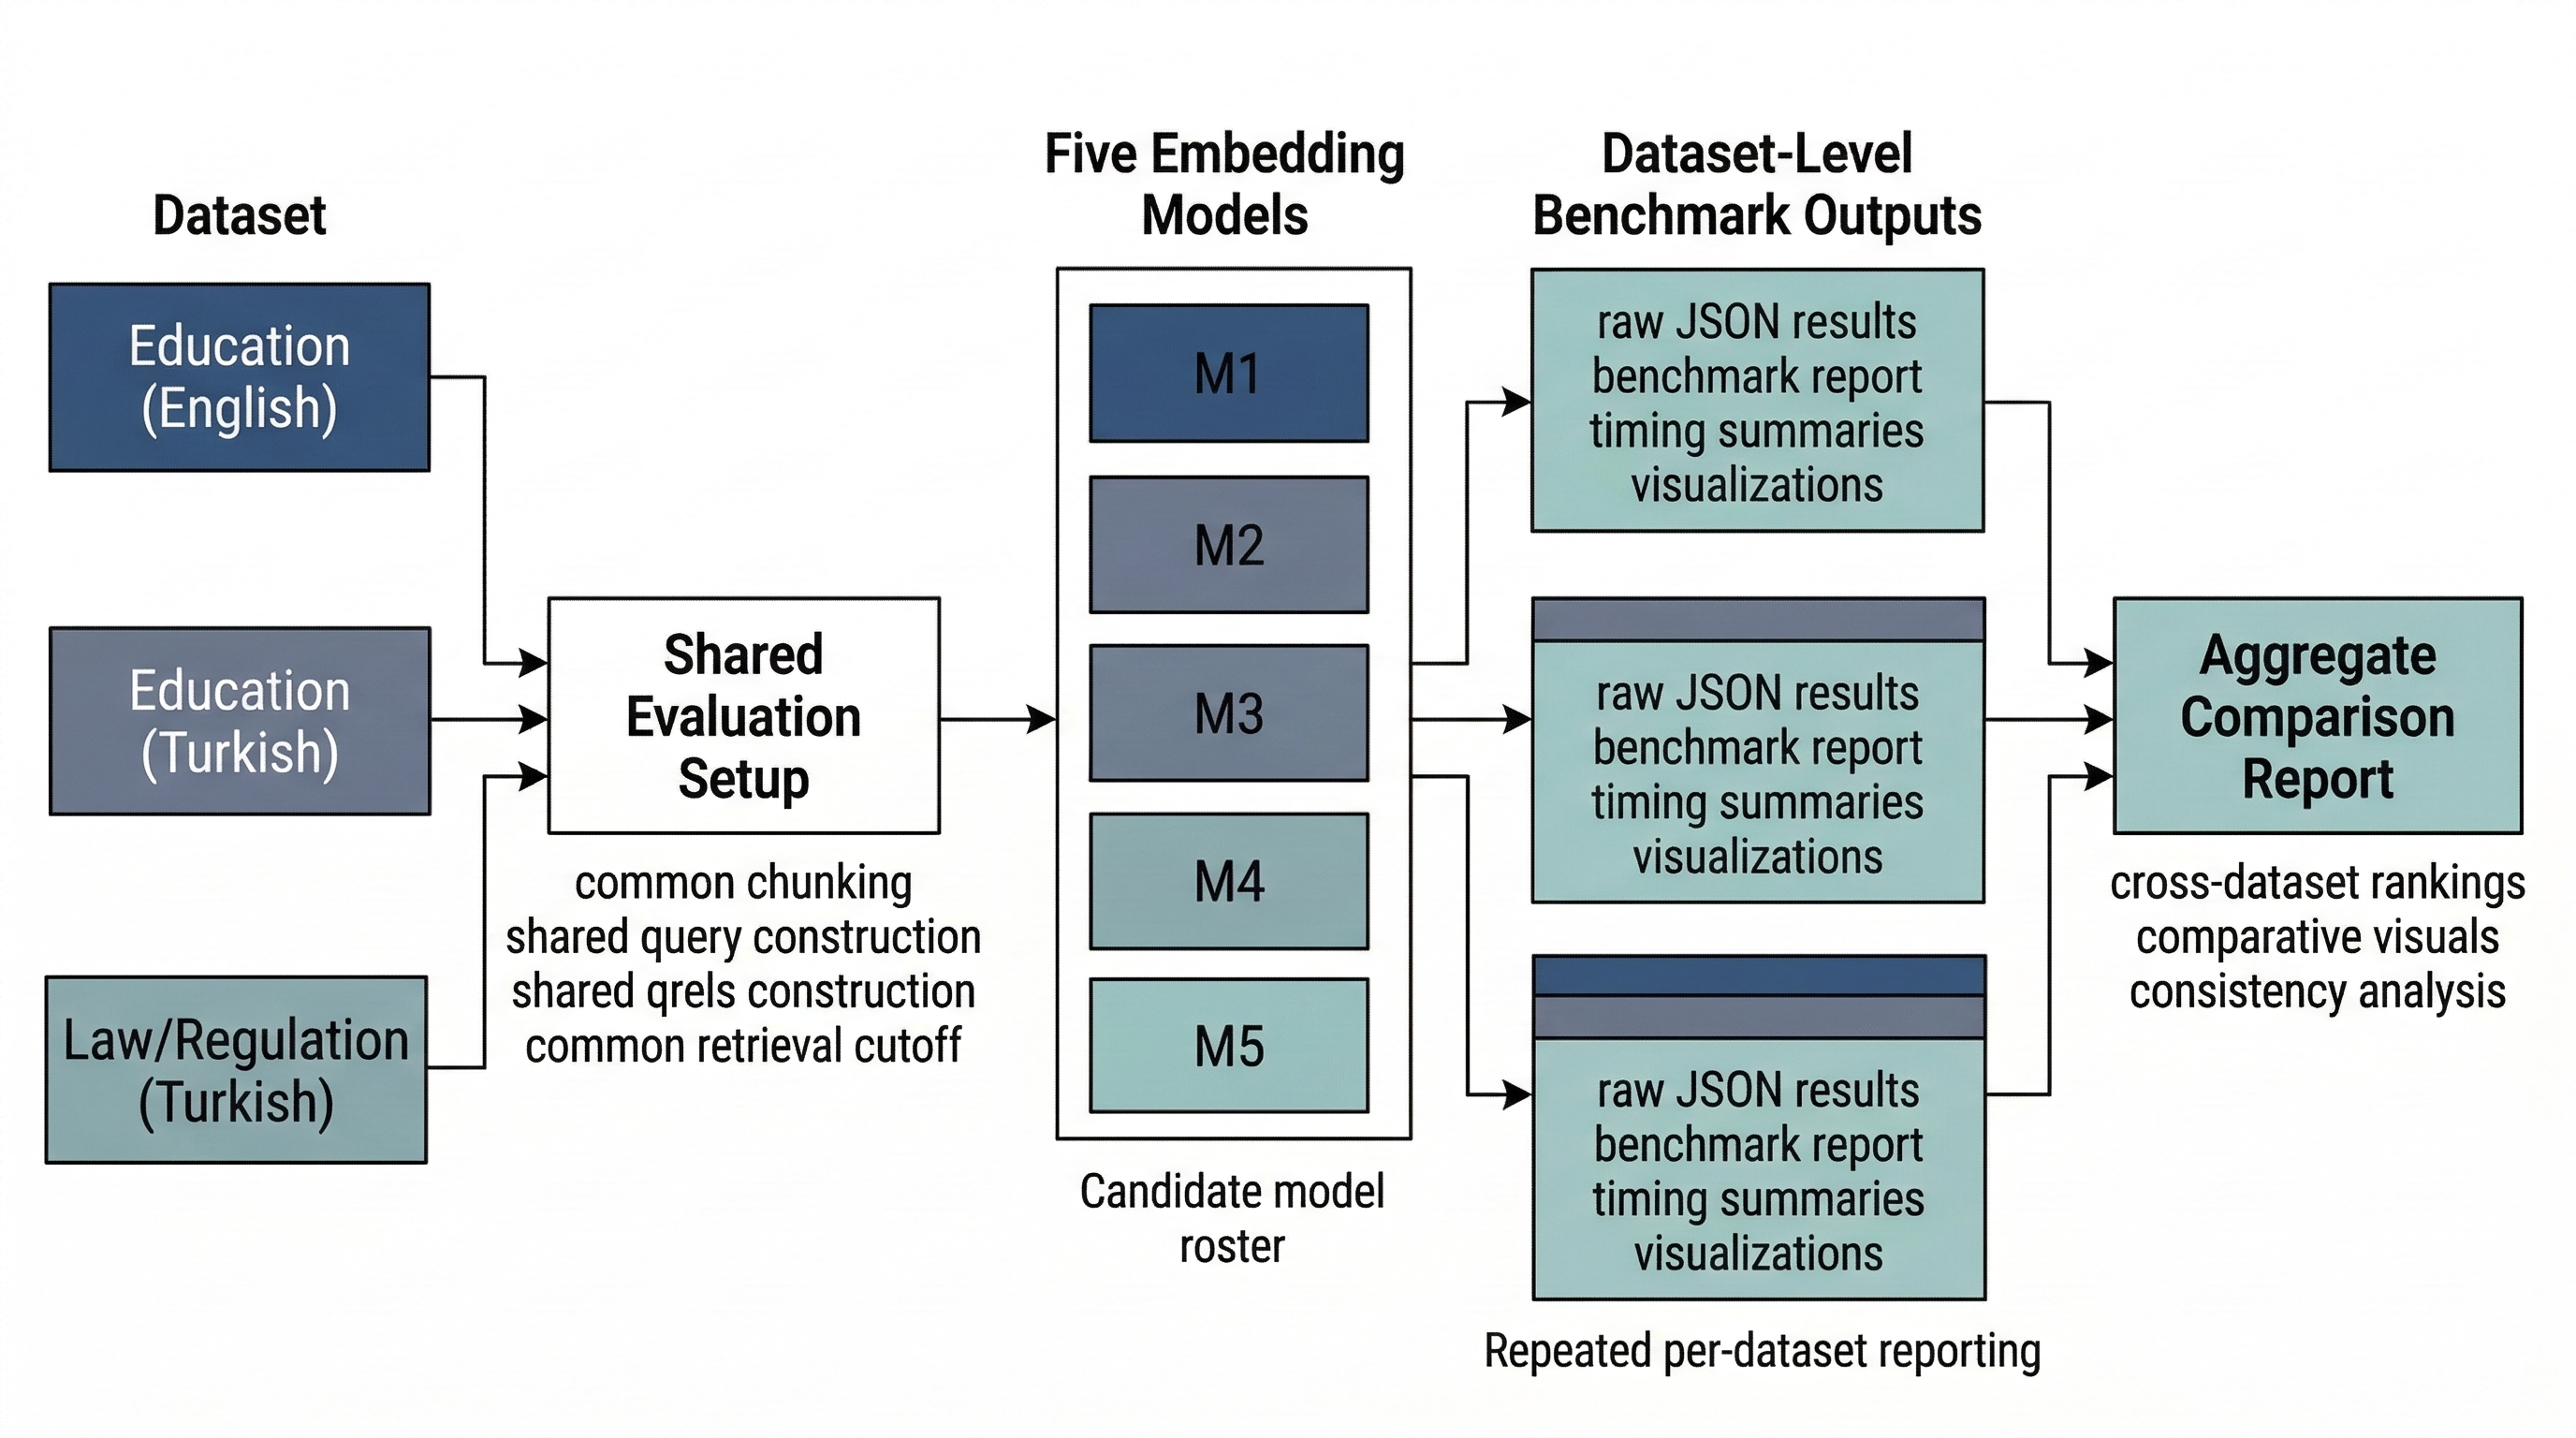
\includegraphics[width=0.95\linewidth]{experimental_design.png}
\caption{Experimental design used to instantiate the proposed benchmarking pipeline in this paper.}\label{fig:experiment_snapshot_design}
\end{figure}

\subsection{Datasets}\label{datasets}

The benchmark covers three local datasets chosen to expose both language variation and domain variation within one controlled setup. Two corpora belong to the education domain and are provided in English and Turkish, whereas the third corpus belongs to the Turkish legal and regulatory domain. For compact reference in the paper, these datasets are denoted as \texttt{education\_eng}, \texttt{education\_tr}, and \texttt{law\_tr}, respectively. This composition allows the same evaluation workflow to be examined across corpora that differ in language, topic, document structure, and corpus scale. Figure~\ref{fig:experiment_dataset_structure} makes this organization explicit by grouping the datasets first by domain and then by language, while also displaying the workload counts associated with each subset. The corresponding quantitative workload summary and source-provenance boundary are reported in Table~\ref{tbl:dataset_statistics_summary} and Table~\ref{tbl:dataset_provenance}, respectively.

Table~\ref{tbl:dataset_statistics_summary} summarizes the same per-dataset counts in tabular form after document ingestion, chunking, synthetic query generation, and qrels construction. The frozen experimental snapshot contains 60 source documents, 1{,}914 chunks, 150 synthetic queries, and 952 positive relevance judgments in total (explicit non-relevant judgments are also stored; see Section~\ref{method}). These counts define the benchmark workload on which the candidate embedding models were evaluated. Taken together, Figure~\ref{fig:experiment_dataset_structure} and Table~\ref{tbl:dataset_statistics_summary} show an important structural characteristic of the benchmark: although \texttt{law\_tr} contains only two source documents, it yields more chunks than either education dataset. The present dataset collection should therefore be read as an intentionally diverse experimental snapshot that combines language, domain, and document-structure variation within one reusable evaluation design. In the present implementation, these source documents were processed from PDF files, but the experimental logic is framed at the document-collection level rather than at one fixed file format.

\begin{table}[t]
\caption{Dataset statistics summary for the frozen experimental snapshot.}\label{tbl:dataset_statistics_summary}
\centering
\begin{tabular}{@{}lrrrr@{}}
\toprule
Dataset & Source documents & Chunks & Queries & Qrels \\
\midrule
education\_eng & 29 & 572 & 50 & 312 \\
education\_tr & 29 & 619 & 50 & 354 \\
law\_tr & 2 & 723 & 50 & 286 \\
Total & 60 & 1914 & 150 & 952 \\
\bottomrule
\end{tabular}
\end{table}

\subsection{Dataset Provenance}\label{dataset-provenance}

Table~\ref{tbl:dataset_provenance} records the provenance boundary of the datasets used in the paper. Its columns summarize the dataset identifier used in this paper, the corresponding language-and-domain category, and the source collection from which the benchmark subset was curated. The education corpora were curated from the TED University regulations and guidelines collection \citep{TED_Regulations}, whereas the law corpus was curated from the BDDK regulations listing \citep{BDDK_Mevzuat}. All source material was retrieved on \texttt{01/01/2026}. The curated benchmark datasets used in this paper are also distributed through the public RagRetrievalBench repository \citep{GitHub_RagRetrievalBench}, which makes the experimental setup directly reusable for follow-up benchmarking studies. Explicit provenance is important because the benchmark is intended as a reusable local evaluation workflow: when the same procedure is applied to a different institutional collection, domain archive, or multilingual document set, the resulting evidence should be interpreted relative to that corpus boundary.

\begin{table}[t]
\caption{Provenance sources for the benchmark datasets used in this paper.}\label{tbl:dataset_provenance}
\centering
\begin{tabular}{@{}>{\raggedright\arraybackslash}p{0.24\linewidth}>{\raggedright\arraybackslash}p{0.26\linewidth}>{\raggedright\arraybackslash}p{0.42\linewidth}@{}}
\toprule
Dataset & Language and domain & Source \\
\midrule
education\_eng & English education & TED University regulations and guidelines \\
education\_tr & Turkish education & TED University regulations and guidelines \\
law\_tr & Turkish law/regulation & BDDK regulations listing \\
\bottomrule
\end{tabular}
\end{table}

The conceptual organization of the benchmark datasets is illustrated in Figure~\ref{fig:experiment_dataset_structure}. This structure is not itself a result; rather, it explains why the present snapshot, together with the workload statistics in Table~\ref{tbl:dataset_statistics_summary}, is suitable for demonstrating both language-sensitive and domain-sensitive use of the benchmarking pipeline.

\begin{figure}
\centering
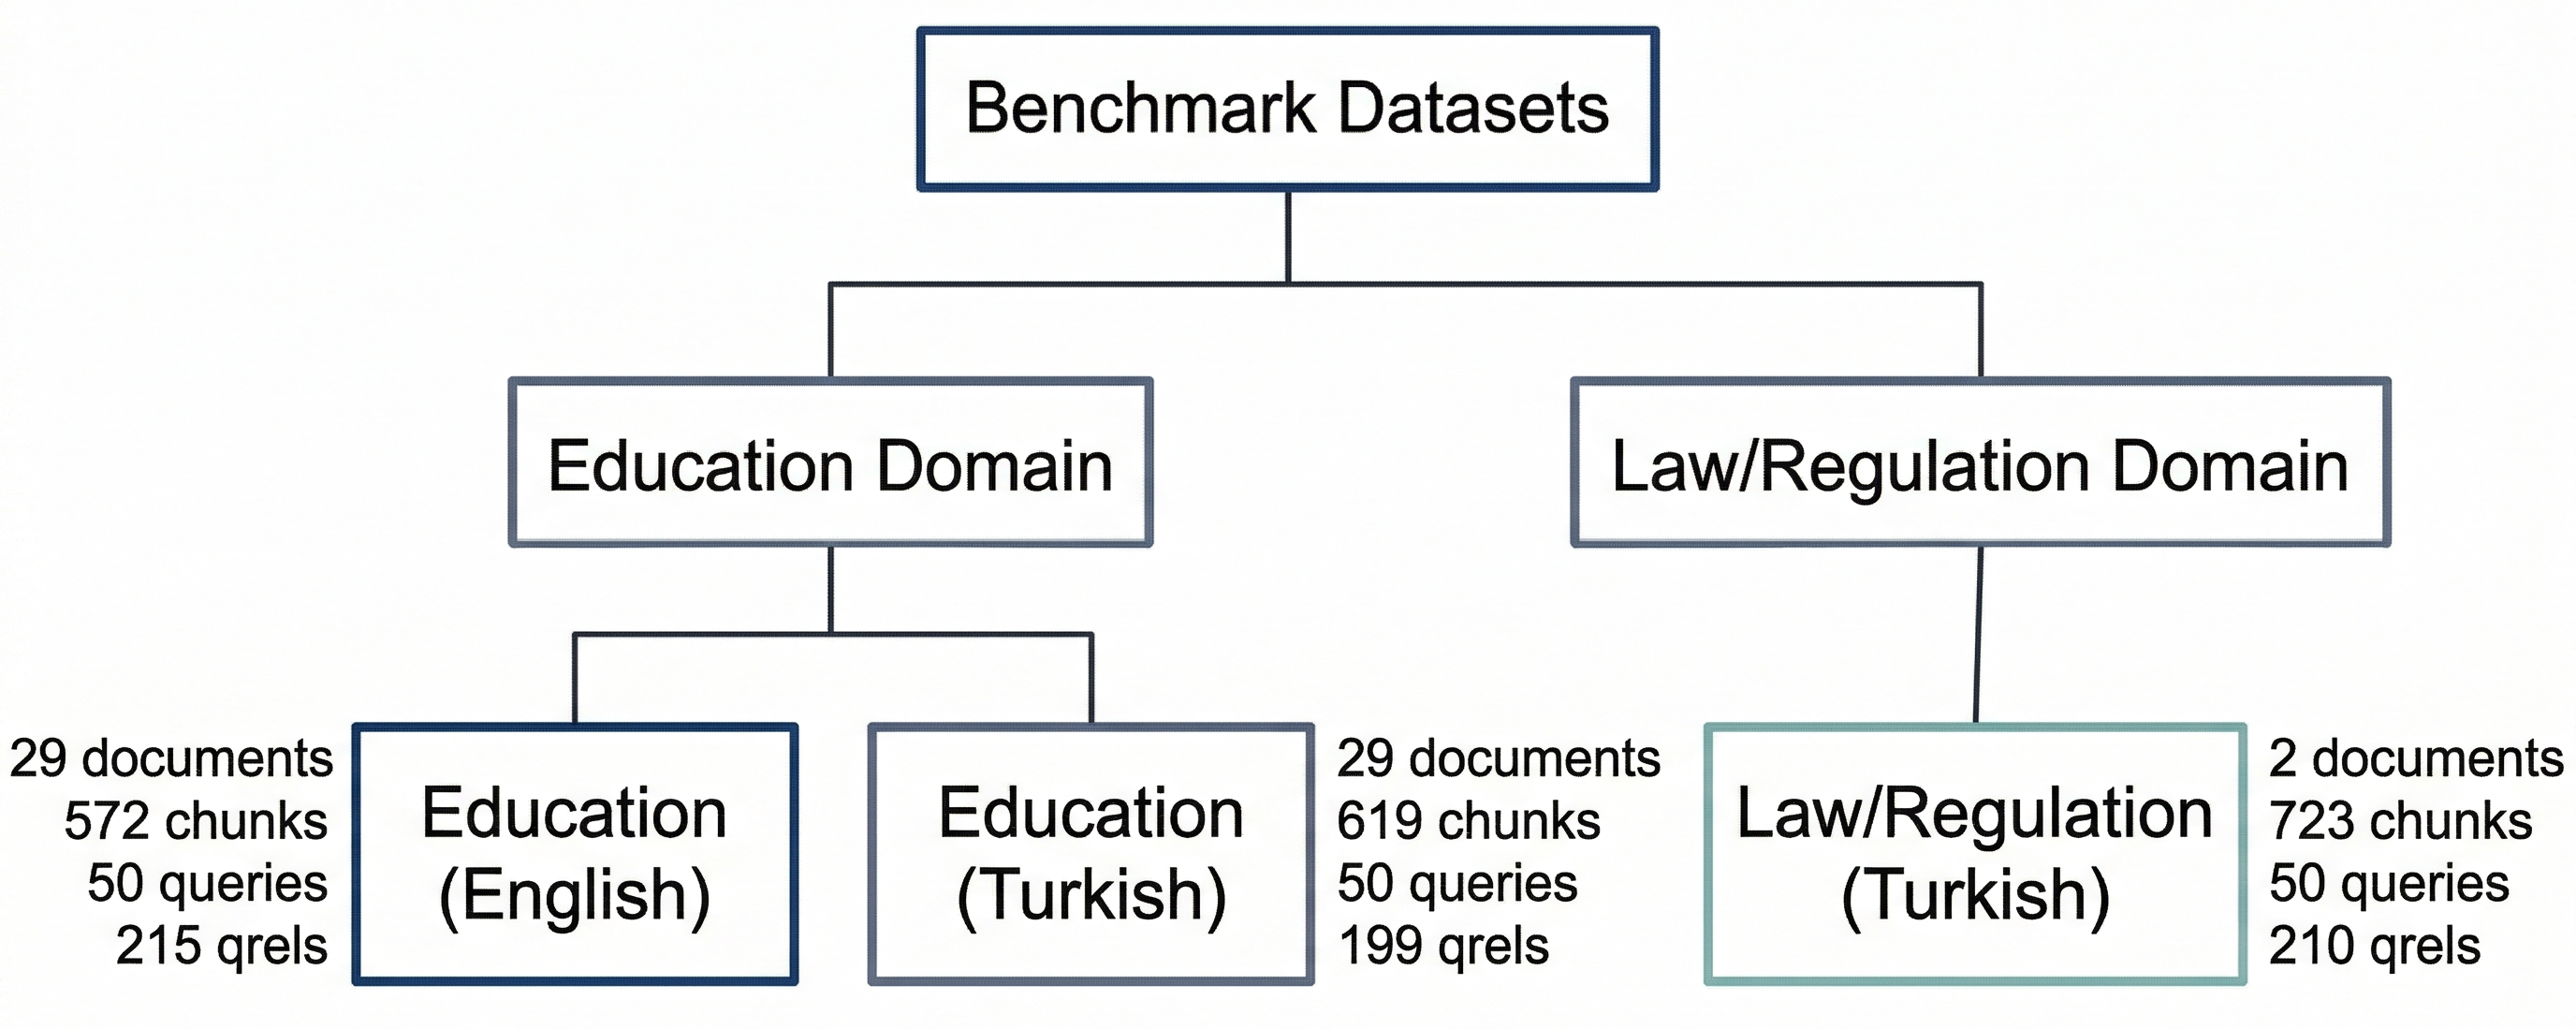
\includegraphics[width=0.95\linewidth]{benchmark_datasets.png}
\caption{Conceptual organization of the benchmark datasets by language and domain, with per-dataset workload counts.}\label{fig:experiment_dataset_structure}
\end{figure}

\subsection{Shared Evaluation Setup}\label{shared-evaluation-setup}

All datasets were processed under the same evaluation configuration so that the main experimental differences arise from corpus characteristics and embedding-model behavior rather than from changes in the benchmark protocol. Retrieval used ChromaDB vector search under its default squared-Euclidean (L2) distance space, with retrieved distances mapped to similarity scores by $1/(1+d)$ for ranking, the common retrieval cutoff was fixed at \texttt{k=10}, chunking used a size of \texttt{1000} characters with \texttt{200} characters of overlap, 50 synthetic queries were generated per dataset, and qrels construction pooled the top-20 candidates retrieved by each of the five models into one model-independent candidate set before LLM judging (Section~\ref{method}). In the pipeline implementation, these experiment-related parameters are stored in a central configuration file, which makes the setup directly accessible and readily adjustable when a practitioner needs to benchmark a different corpus, alternative model roster, or modified operating constraint \citep{ChromaDB_Docs,GitHub_RagRetrievalBench}. This design choice supports the practical aim of the pipeline: the same benchmarking procedure can be adopted as a baseline configuration and then adapted systematically to corpus-specific requirements without changing the overall evaluation logic. Table~\ref{tbl:experiment_workflow_parameters} summarizes the fixed parameter values that define this shared setup across chunking, query construction, index creation, and retrieval evaluation. These values are demonstration-scale defaults rather than tuned optima: 50 queries per dataset, a candidate pool of 20, a chunk size of 1000 characters with 200 of overlap, and a retrieval cutoff of \texttt{k=10} follow common practitioner defaults and the repository's baseline configuration. They are held fixed here so that differences arise from corpus and model rather than from the protocol, and they are exposed as editable configuration; their sensitivity is examined as future work (Section~\ref{conclusion}) rather than claimed to be optimal.

For the present experimental snapshot, synthetic query generation and qrels construction both used the Gemini 2.5 Flash-Lite model. More specifically, the pipeline applies the same LLM family in two roles: first to synthesize a source-language query from each selected seed chunk, and then to act as a binary relevance judge over the retrieved candidate chunks associated with that query. The pipeline supports two operational modes for these LLM-dependent stages. A practitioner may run them through immediate request--response interaction when the benchmark is small or iterative inspection is desired, or may submit them through a batch-processing workflow that separates job submission from result retrieval and can reduce the total cost of larger benchmark runs. This dual execution design improves operational flexibility because the same benchmark logic can be retained while the execution mode is adapted to dataset size, budget, or turnaround constraints \citep{GitHub_RagRetrievalBench}.

\begin{table}[t]
\caption{Fixed workflow parameters used in the shared experimental configuration.}\label{tbl:experiment_workflow_parameters}
\centering
\small
\begin{tabular}{@{}>{\raggedright\arraybackslash}p{0.24\linewidth}>{\raggedright\arraybackslash}p{0.13\linewidth}>{\raggedright\arraybackslash}p{0.51\linewidth}@{}}
\toprule
Parameter & Value & Role in the workflow \\
\midrule
Chunk size & 1000 & Determines the maximum character length of each corpus segment before embedding \\
Chunk overlap & 200 & Preserves continuity between adjacent chunks and reduces boundary-induced information loss \\
Queries per dataset & 50 & Fixes the size of the synthetic evaluation set generated for each corpus \\
Chunks per query seed & 1 & Anchors each generated query to one sampled source chunk during query construction \\
Candidate pool size & 20 & Limits the number of retrieved candidates examined during relevance construction \\
Document batch size & 32 & Controls batched embedding throughput during vector collection construction \\
Collection reinitialization & True & Rebuilds vector collections so each benchmark run starts from a controlled index state \\
Shared retrieval cutoff & 10 & Fixes the number of ranked chunks returned per query during retrieval evaluation \\
\bottomrule
\end{tabular}
\end{table}

Table~\ref{tbl:experiment_embedding_models} lists the embedding model roster used in the experimental configuration. The table identifies each model, its embedding dimension, and its role within the benchmarked roster. This model family was selected because the Sentence Transformers project provides openly available and widely adopted embedding models together with stable documentation and reproducible usage patterns for semantic search applications \citep{SentenceTransformers_Website}. In addition, the five models benchmarked in this paper were selected from among the most downloaded models listed in the Sentence Transformers Hugging Face repository, which makes them representative of models that practitioners are likely to consider first when assembling an open embedding baseline \citep{SentenceTransformers_HF_Repo,HuggingFace_SentenceTransformers}. The purpose of the present setup is not to claim that the sentence-transformer family exhausts all relevant embedding choices; rather, it is to demonstrate that the proposed pipeline can evaluate a realistic candidate set under controlled conditions using models that are directly accessible to practitioners and straightforward to reproduce. Because the pipeline is implemented as an open and configurable workflow, the same procedure can be extended to embedding models from other providers when a different deployment requirement or procurement constraint must be studied. For the practical objective of this paper, however, the selected open-weight models provide a sufficient and reproducible test bed for demonstrating the effectiveness of the benchmarking pipeline itself.

\begin{table}[t]
\caption{Embedding model roster used in the experimental configuration.}\label{tbl:experiment_embedding_models}
\centering
\small
\begin{tabular}{@{}>{\raggedright\arraybackslash}p{0.08\linewidth}>{\raggedright\arraybackslash}p{0.44\linewidth}>{\raggedright\arraybackslash}p{0.12\linewidth}>{\raggedright\arraybackslash}p{0.26\linewidth}@{}}
\toprule
ID & Model & Dimension & Role in the benchmark \\
\midrule
M1 & sentence-transformers/all-MiniLM-L6-v2 & 384 & English-trained MiniLM; lightweight efficiency baseline \\
M2 & sentence-transformers/all-mpnet-base-v2 & 768 & English-trained MPNet; higher-capacity English-oriented model \\
M3 & sentence-transformers/paraphrase-multilingual-MiniLM-L12-v2 & 384 & Multilingual (paraphrase) MiniLM; compact cross-language model \\
M4 & sentence-transformers/all-MiniLM-L12-v2 & 384 & English-trained MiniLM; deeper L12 variant \\
M5 & sentence-transformers/paraphrase-multilingual-mpnet-base-v2 & 768 & Multilingual (paraphrase) MPNet; higher-capacity cross-language model \\
\bottomrule
\end{tabular}
\end{table}

Throughout the paper, \emph{English-oriented} (used interchangeably with monolingual) is shorthand for the \texttt{all-MiniLM} and \texttt{all-mpnet} models, which are trained predominantly on English data, while \emph{multilingual} denotes the \texttt{paraphrase-multilingual} models, which are trained on many languages. These labels describe the intended training regime and are used for discussion; they are not strict claims about tokenizer coverage or guaranteed per-language quality.

To preserve comparability across datasets, the experiments held constant the metric definitions and retrieval cutoff, the embedding model roster, the candidate pool size used during qrels construction, the chunking parameters summarized in Table~\ref{tbl:experiment_workflow_parameters}, and the reporting pipeline. The intentionally varying factors were corpus language, domain, corpus size, and document composition. This separation between fixed and varying factors provides a practical guideline for external reuse: a practitioner who wishes to benchmark a different corpus can keep the evaluation frame fixed while substituting a new dataset collection and, if needed, a different candidate model list.

\subsection{Reproducibility Conditions}\label{reproducibility-conditions}

Table~\ref{tbl:reproducibility} summarizes the software, data-processing, and measurement conditions required to reproduce the benchmark; library versions are pinned in the public repository \citep{GitHub_RagRetrievalBench}. Seed-chunk sampling uses a fixed random seed, and each run records an environment snapshot (Python and library versions, device) in its raw-result JSON, so the reported snapshot is reproducible from the released corpus, queries, and qrels. One condition remains a genuine limitation: the reported runs were executed on CPU without a controlled hardware matrix, so the timing measurements should be read as relative, same-machine comparisons between models rather than as absolute, machine-transferable latencies.

\begin{table}[t]
\caption{Reproducibility conditions for the benchmark snapshot.}\label{tbl:reproducibility}
\centering
\small
\begin{tabular}{@{}>{\raggedright\arraybackslash}p{0.30\linewidth}>{\raggedright\arraybackslash}p{0.62\linewidth}@{}}
\toprule
Component & Setting \\
\midrule
Language runtime & Python 3.10 (\texttt{ragbenchmark} conda environment) \\
Vector store & ChromaDB 1.0.7 (persistent client), default squared-Euclidean (L2) space; similarity $1/(1+d)$ \\
Embeddings & Sentence-Transformers 4.1.0 (PyTorch 2.7.0), default non-normalized encoding, batch size 32 \\
Text extraction & PyMuPDF 1.26.0 page text with NFC Unicode normalization \\
Chunking & LangChain recursive character splitter, size 1000, overlap 200 \\
Retrieval evaluation & Sentence-Transformers \texttt{InformationRetrievalEvaluator}, cutoff $k=10$ \\
Query generation and judging & Gemini 2.5 Flash-Lite, temperature 0.1, in batch and interactive modes \\
Candidate pool & Model-independent union of the top-20 chunks retrieved by all five models, LLM-judged with stored positive and negative labels; a single-model (\texttt{M5}-only) variant is compared in Section~\ref{results} \\
Seed policy & Fixed random seed (42) for seed-chunk sampling, so the reported snapshot is reproducible \\
Timing scope & Query latency $=$ query embedding $+$ vector search (local only, measured cold, no LLM or network); embedding time $=$ batched corpus embedding and insertion \\
Hardware / OS / device & Environment snapshot (Python and library versions, device) recorded in each raw-result JSON; the reported runs used CPU, so timing is single-machine and should be read as relative \\
Released artifacts & Corpus, queries, qrels, raw-result JSON, and reports in the public repository \citep{GitHub_RagRetrievalBench} \\
\bottomrule
\end{tabular}
\end{table}

\subsection{Report Outputs and Utility}\label{report-outputs-and-utility}

The reporting outputs generated in these experiments follow the two-layer reporting design described in Section~\ref{automated-reporting-and-reproducibility}, Figure~\ref{fig:method_reporting_workflow}, and Table~\ref{tbl:method_reporting_outputs}. For each dataset run, the pipeline first materializes the evaluation state as a machine-readable raw-result JSON artifact. These stored results preserve the essential benchmark record, including the applied configuration, corpus and query statistics, qrels characteristics, per-model retrieval scores, and timing measurements. This design is important for practical reuse because the underlying experimental evidence remains available for later verification, archival reference, re-analysis, or downstream comparison without requiring the retrieval workflow to be executed again.

The human-readable benchmark reports are then generated from these stored JSON results rather than from transient console output. At the dataset level, the pipeline produces a benchmark report together with ranking summaries, timing summaries, and visualization assets covering metric profiles, ranking comparisons, consistency patterns, and timing behavior. This separation between raw-result storage and report generation makes the setup easier to reuse in practice: a practitioner can preserve the original benchmark evidence, regenerate presentation-oriented summaries when needed, and inspect one dataset or one representative subset as a self-contained decision-support case.

When multiple dataset runs are available, the aggregate reporting stage loads the dataset-level JSON artifacts and constructs a cross-dataset comparison report with comparative visual summaries. In the present paper, this second reporting layer provides the experimental basis for comparing embedding behavior across language- and domain-differentiated subsets under one shared setup. Within the experimental section, these reporting products are operational outputs of the benchmark procedure rather than findings in themselves. The substantive comparative evidence derived from them is presented separately in Section~\ref{results}.
